  %%%%%%%%%%%%%%%%%%%%%%%%%%%%%%%%%%%%%%% -*- coding: utf-8; mode: latex -*- %%
  %
%%%%%                         CHAPTER
 %%%
  %

% $Id: 2200-irure-dolor.tex,v 1.1 2007/11/23 09:52:42 david Exp $
% $Log: 2200-irure-dolor.tex,v $
% Revision 1.1  2007/11/23 09:52:42  david
% *** empty log message ***
%
%

  %%%%%%%%%%%%%%%%%%%%%%%%%%%%%%%%%%%%%%%%%%%%%%%%%%%%%%%%%%%%%%%%%%%%%%%%%%%%%
  %
%%%%%                     HEAD MATTER
 %%%
  %

\chapter{Namespace Locking}
%\addcontentsline{lof}{chapter}{\thechapter\quad Irure Dolor}
%\addcontentsline{lot}{chapter}{\thechapter\quad Irure Dolor}
\label{ch:Locking}

%\begin{quotation}
%  {\small\it Neque porro quisquam est qui dolorem ipsum quia dolor sit amet, consectetur, adipisci velit...}
%
%{\small\it -- Cerico}
%\end{quotation}

\subsection{The Namespace Locking in GFS}

Unlike traditional file systems, GFS doesn't have a per-directory data structure, which means that it doesn't support listing all files in a directory (i.e, \textit{ls} in POSIX), nor aliasing for the same file or directory (i.e, hard or symbolic links). Instead, with prefix compression, GFS represents the namespace as a lookup table mapping full pathnames to metadata logically. Therefore, each node in the namespace tree will be associated a \textit{read-write} lock. To prevent deadlock, locks are acquired in a \textit{consistent total order}: first ordered by level, then ordered lexicographically within the same level~\cite{ghemawat2003google}.

\noindent One benefit for the locking scheme in GFS is that it allows concurrent mutations for different files/directories within the same directory. 

\begin{figure}[ht]
	\centering
	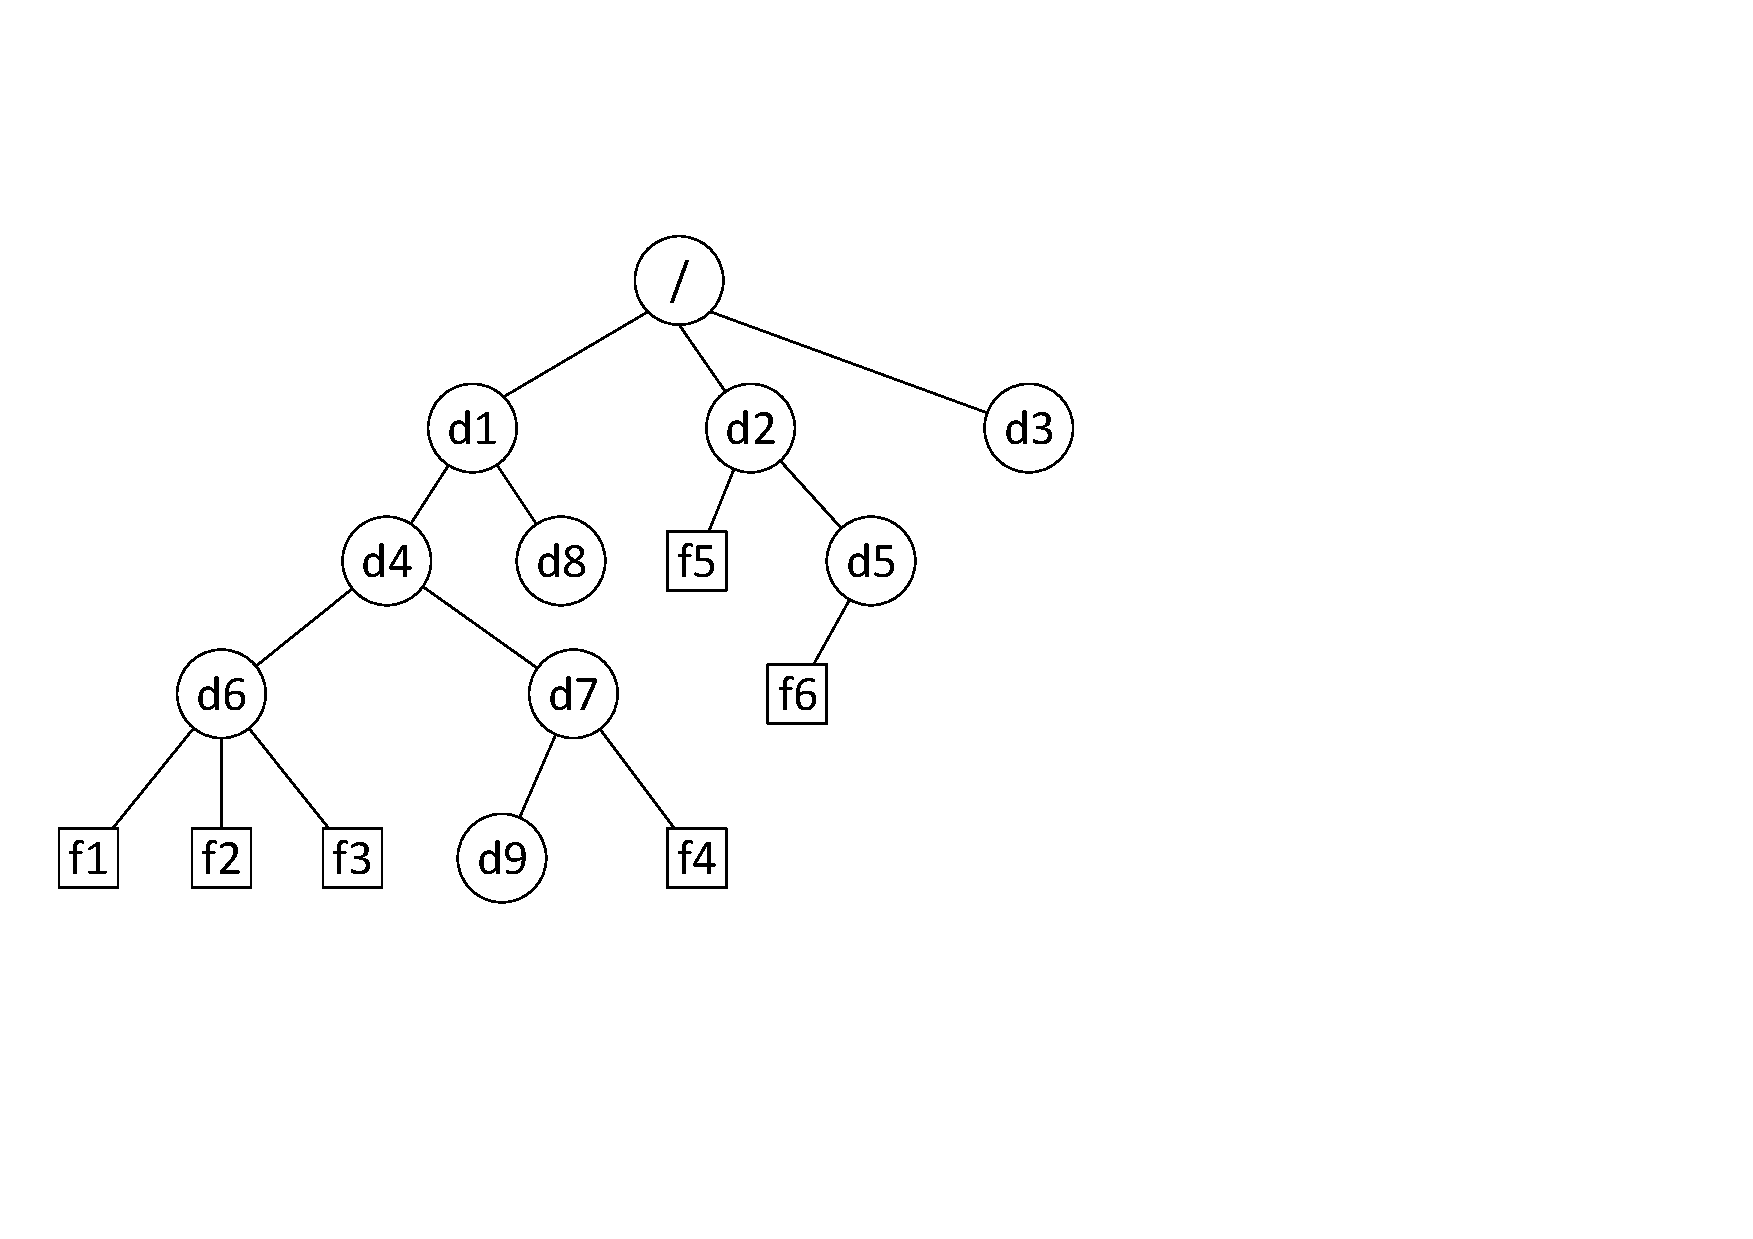
\includegraphics[scale=0.7]{figs/gfstree.pdf}
	\caption{A Graphical Tree Representation for the Namespace in GFS}
	\label{fig:gfsTree}
\end{figure}

\noindent For example, suppose that we have a graphical tree representation for the namespace in GFS as shown in Figure~\ref{fig:gfsTree}. Concurrently, we have five operations involving files \textit{f1, f2, f3, f4} and directory \textit{d9}. As we can see from Table~\ref{table:gfsLock1}, there are no conflicting locks (\textit{Read-Write and Write-Write}), all these five operations are all allowed to happen concurrently.

\begin{table}
	\centering
    \begin{tabular}{|l|c|c|c|c|c|}
    	\hline
    	\textbf{\textit{Total Order Locks}}            & \textbf{Operation1} & \textbf{Operation2} & \textbf{Operation3} & \textbf{Operation4} & \textbf{Operation5} \\ \hline
    	\textbf{\color{red}/ }           & Read1      & Read2      & Read3      & Read4      & Read5      \\ \hline
    	/\textbf{\color{red}d1}          & Read1      & Read2      & Read3      & Read4      & Read5      \\ \hline
    	/d1/\textbf{\color{red}d4}       & Read1      & Read2      & Read3      & Read4      & Read5      \\ \hline
    	/d1/d4/\textbf{\color{red}d6}    & Read1      & Read2      & Read3      & ~          & ~          \\ \hline
    	/d1/d4/\textbf{\color{red}d7}    & ~          & ~          & ~          & Read4      & Read5      \\ \hline
    	/d1/d4/d6/\textbf{\color{red}f1} & Write1     & ~          & ~          & ~          & ~          \\ \hline
    	/d1/d4/d6/\textbf{\color{red}f2} & ~          & Write2     & ~          & ~          & ~          \\ \hline
    	/d1/d4/d6/\textbf{\color{red}f3} & ~          & ~          & Write3     & ~          & ~          \\ \hline
    	/d1/d4/d7/\textbf{\color{red}d9} & ~          & ~          & ~          & Write4     & Write5     \\ \hline
    	/d1/d4/d7/\textbf{\color{red}f4} & ~          & ~          & ~          & ~          & ~          \\ \hline
    \end{tabular}
	\caption{Concurrent Mutations within for different files/directories and Related Read-Write Lock Sets}
	\label{table:gfsLock1}
\end{table}

\noindent Since operations will be serialized properly when trying to obtain conflict locks(\textit{Read-Write and Write-Write}), concurrent mutations on the same file/directory will be prevented.

\begin{table}[ht]
	\centering
	\begin{tabular}{|l|c|c|}
		\hline
		\textbf{\textit{Total Order Locks}}             & \textbf{Operation1} & \textbf{Operation2}                    \\ \hline
		\textbf{\color{red}/}             & Read1      & Read2                         \\ \hline
		/\textbf{\color{red}d1}           & Read1      & Read2                         \\ \hline
		/\textbf{\color{red}d3}           & Read1      & ~                             \\ \hline
		/d1/\textbf{\color{red}d8}        & Write1     & Read2 \textbf{(Conflicts with Write1)} \\ \hline
		/d3/\textbf{\color{red}d8}       & Write1     & ~                             \\ \hline
		/d1/d8/\textbf{\color{red}Qi.txt} & ~          & Write2                        \\ \hline
	\end{tabular}
	\caption{Serialized Concurrent Mutations and Conflict Locks}
	\label{table:gfsLock2}
\end{table}

\noindent For example, if there are another two concurrent operations. \textit{Operation 1} wants to snapshot directory \textit{d8} to be under directory \textit{d3}, but \textit{Operation 2} wants to create a new file \textit{Qi.txt} under directory \textit{d8}. Table~\ref{table:gfsLock2} shows how conflict locks prevent the new file \textit{Qi.txt} being created when directory \textit{d8} is being snapshotting.

  %%%%%%%%%%%%%%%%%%%%%%%%%%%%%%%%%%%%%%%%%%%%%%%%%%%%%%%%%%%%%%%%%%%%%%%%%%%%%
  %
%%%%%                        FIRST SECTION
 %%%
  %

\section{A}




  %%%%%%%%%%%%%%%%%%%%%%%%%%%%%%%%%%%%%%%%%%%%%%%%%%%%%%%%%%%%%%%%%%%%%%%%%%%%%
  %
%%%%%                      SECOND SECTION
 %%%
  %

\section{B}


  %%%%%%%%%%%%%%%%%%%%%%%%%%%%%%%%%%%%%%%%%%%%%%%%%%%%%%%%%%%%%%%%%%%%%%%%%%%%%
  %
%%%%%                         ANOTHER SECTION
 %%%
  %
\section{C}

CCC

  %%%%%%%%%%%%%%%%%%%%%%%%%%%%%%%%%%%%%%%%%%%%%%%%%%%%%%%%%%%%%%%%%%%%%%%%%%%%%
  %
%%%%%                          LAST SECTION
 %%%
  %

\section{D}

DDD

  %
 %%%
%%%%%                           THE END
  %
  %%%%%%%%%%%%%%%%%%%%%%%%%%%%%%%%%%%%%%%%%%%%%%%%%%%%%%%%%%%%%%%%%%%%%%%%%%%%%

%%% Local Variables: 
%%% mode: latex
%%% TeX-master: "tese"
%%% End: 
